\chapter{Memory BIST Fundamentals}
\label{chap:background}
Memory testing has many components.  The basic concept is to confirm that a value written to a memory address is still present in that memory address at any point in the future.  Many factors can affect the ability of the memory to retain its proper value.  Those factors manifest as one of the four standard memory faults: Stuck-At Faults, Transitional Faults, Coupling Faults and Neighborhood Pattern-Sensitive Faults \cite{VanDeGoor1991}. All current BIST engines are able to detect these faults with varying degrees of effectiveness.

The BIST engines use memory test algorithms to detect, and in some cases, repair these faults. The common tests used in industry ar  

A major influence to the test algorithmThe address counting method and address order have major influences to a test algorithm's ability to detect these faults.   A BIST needs an address generator that can produce the correct sequence of addresses without omitting any addresses.  

\section{Memory Faults}
\label{sect:bg-faults}
Precise fault modeling is the key to designing efficient fault tests.  Fault models reflect real, specific defects in memory so high defect coverage and detection is strongly dependent on the quality of the fault model \cite{1327984}.  The following sections offer a brief description about the four classic types of faults \cite{Adams2003} that models are designed to detect.  

\subsection{Stuck-At Faults}
The most common type of memory fault occurs when the memory cell is locked into one state, either a “0” or “1”.  A defect free cell can be written to either state and, when read, will still contain the information previously written.  The stuck-at fault occurs when a state is written to the cell, but the subsequent reads return the only one state regardless of the previously written value.  Fig. 2 shows the state diagram for a stuck-at fault \cite{oldref-03}.
Another fault that can be classified as a stuck-at fault is the address decoder fault.  It is like the data stuck-at fault, but occurs on the address lines and leads to accessing wrong addresses, no addresses, or multiple addresses \cite{oldref-03}.

\subsection{Transitional Faults}
Similar to a stuck-at fault, the transition fault also locks into a single state, but has the characteristic of being in either state prior to the write.  The memory cell may contain “0” or “1” when powered on, but after a write, it cannot transition back.  The characteristic behavior of this fault is the memory can only written in one direction.  

\subsection{Coupling Faults}
There are numerous types of coupling faults, but they can be simply expressed as a cell affecting its neighboring cells and causing the neighbor to falsely transition or change state.  Coupling faults can be unidirectional or bi-directional.  In unidirectional coupling faults, one cell (aggressor cell) couples into another (victim cell), but the opposite does not occur.  A parasitic diode connection between the cells is a common cause of this behavior.  The bi-directional coupling fault occurs when pairs of cells can affect each other.  One way that this type of defect can occur is through bridging \cite{Adams2003}.  

\subsection{Neighborhood Pattern-Sensitive Fault (NPSF)}
\label{sec:npsf}
This fault model is in the class of coupling faults, but it is caused by particular patterns in neighboring cells rather than one specific cell.  The neighborhoods are usually defined as Type-1 or Type-2 neighborhoods \cite{1047051} as shown in Figure \ref{fig:npsftypes}.  Type-1 neighborhoods consist of five cells: one cell in center and four cells physically adjacent to the center cell.  In this configuration, the center cell is the base cell and the four adjacent cells are called the deleted neighborhood.  Type-2 neighborhoods consist of multiple cells where the base cell is in the center and deleted neighborhood is comprised of the cells within $m_1$ columns to the left, $m_2$ rows above, $m_3$ columns to the right and $m_4$ rows below the base cell.  This report will focus on Type-1 neighborhoods.

\begin{figure}[h!]
  \centering
  \begin{subfigure}[b]{0.4\textwidth}
    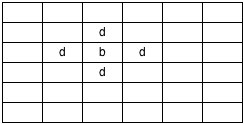
\includegraphics[width=\textwidth]{type1}
    \caption{Type-1 Neighborhood}
    \label{fig:type1}
  \end{subfigure}
  \begin{subfigure}[b]{0.4\textwidth}
    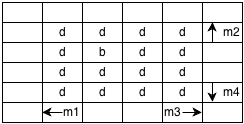
\includegraphics[width=\textwidth]{type2}
    \caption{Type-2 Neighborhood}
    \label{fig:type2}
  \end{subfigure}
  \caption{NPSF Neighborhoods \\
           b: base cell \\
           d: deleted neighborhood} 
           %$m_1$ = $m_2$ = 1; $m_3$ = $m_4$ = 2}
  \label{fig:npsftypes}
\end{figure}

Three classes of NPSF faults exist:
\begin{enumerate}
  \item Active NPSF (ANPSF): the base cell's contents change due to changes in the pattern of the deleted neighborhood.
  \item Passive NPSF (PNPSF): the base cell's contents cannot change due to specific pattern in the deleted neighborhood.
  \item Static NPSF (SNPSF): the base cell's contents are forced to a specific value because of the contents of the deleted neighborhood
\end{enumerate}

To test for all three classes of NPSF faults, all the combinations of values in the deleted cells and their transitions must be performed against the base cell.  To do this, a Eulerian Sequence is employed to generate the appropriate sequence of values in the neighborhood.  \cite{1675556} offers a proof of the Eulerian Sequence as a testing mechanism.  A 5-bit Eulerian Sequence is used as the Type-1 pattern.

To reduce the number of write operations to memory, multiple patterns can be written to memory simultaneously using either the tiling or two-group methods as shown in Figure \ref{fig:type1methods}.

\begin{figure}[h]
  \centering
  
\includegraphics[width=\textwidth]{placeholder}
  \caption{Type-1 with tiling method and two-group method}
  \label{fig:type1methods}
\end{figure}

In the tiling method, each tile is written to memory is such a way that none of the tiles overlap.  The two-group method is comprised to two checkerboard patterns that are overlaid is such a way that a base cell is in one checkerboard pattern while the deleted neighborhood is within the other checkerboard pattern.  This report will use the tiling method.

\section{Memory Test Algorithms}
\label{sect:bg-algorithms}
The early tests before the 1980`s were not based on fault models or proofs.  Tests of this time, such as Scan, GALPAT and Walking, were considered ad-hoc and usually have very long test times of order \textit{O(n\textsuperscript{2})} making the non-ideal for larger memories \cite{1327984}.  The introduction of fault models in the early 1980`s allowed the fault coverage to be mathematically proven.  This paved the way for March tests to become the dominant type of tests since their fault coverage is proven mathematically and test time is linearly related to the size of the memory \cite{1327984}.  

\subsection{GALPAT and variations}
The GALPAT or Galloping 1’s and 0’s algorithm sequences through all memory addresses to test for faults.  It starts by writing a background of zeros into all memory cells, then complements the first cell and compares it to every other cell, reading the base and test cell every time.  The test continues testing every cell by complementing the current cell and comparing it to every other cell \cite{oldref-09}.  The test is effective for finding stuck-at faults, coupling faults and transition faults, but suffers from an extremely long test time compared to march tests \cite{1327984}.  


\subsection{Walking Algorithms}
Walking algorithms are similar to GALPAT tests.  They begin by initializing all memory to zeros and then complement the first test cell, or base cell.  The test reads the base cell and then reads each of the memory cells to compare results without re-reading the base cell.  The test is effective at finding SAF, but suffers from test times proportional to \textit{O(n\textsuperscript{2})} \cite{VanDeGoor1991}.  


\subsection{March Test}
The March test has become the most popular testing algorithm for memory.  The March test algorithm is a finite sequence of March Elements (ME), each of which can be shared between other algorithms.  A ME specifies the sequence of actions, or March operations (MO), applied to each cell before proceeding to the next cell \cite{199799}.  The MO is the action performed at the memory cell: write a 0 (w0), write a 1 (w1), read a zero (r0) and read a 1 (r1) \cite{199799}.

The order in which the memory addresses are tested is the address order (AO), and the actual sequence of addresses is the counting method (CM).  For example, for the range 1\ldots10, the sequence 1,2,3,\ldots,9,10 would have an ascending AO and linear CM.  Conversely, 10,9,\ldots,3,2,1 would have a descending AO and a linear CM. The AO uses the symbols $\Uparrow$ (ascending),$\Downarrow$ (descending),$\Updownarrow$ (AO irrelevant) as abbreviations in the ME definition \cite{199799}.

The ME ‘$\Updownarrow$(r0,w1)’, is interpreted at each memory address as read the memory with expected value of \textit{0}, write a value of \textit{1} and continue to the next address in ascending order \cite{5491773}.    









\section{Memory Address Counting Methods}
\label{sect:bg-counting}
For any number \textit{N}, there are \textit{N}! ways to count to \textit{N}.  The memory address counting methods are important because they can directly affect a test's effectiveness at detecting faults.  Running the test with all possible CM (\textit{N}!) is not practical with today's memory sizes, so designers must use innovative CM that reduce test time while achieving maximum test coverage.  The address generator in this report will focus on CM that are common and important.  Each of the CM included has its own fault detection capability \cite{1347645}, \cite{990255}, \cite{1584048}, \cite{5359299}, \cite{1576336}.  Table \ref{tab:cm} provides an example of each CM for a four-bit address line.

\begin{table}[H]
  \caption{Address Counting Methods}
  \centering
  \begin{tabular}{|c|c|c|c|c|c|}
  \hline
  %heading
  Step & LI & AC   & GC & 2\textsuperscript{\textit{i}}=4 & PR \\
  \hline\hline
   0 & 0000 & 0000 & 0000 & 0000 & 0000 \\ 
   1 & 0001 & 1111 & 0001 & 0100 & 0001 \\ 
   2 & 0010 & 0001 & 0011 & 1000 & 0011 \\ 
   3 & 0011 & 1110 & 0010 & 1100 & 0111 \\ 
   \hline
   4 & 0100 & 0010 & 0110 & 0001 & 1111 \\ 
   5 & 0101 & 1101 & 0111 & 0101 & 1110 \\ 
   6 & 0110 & 0011 & 0101 & 1001 & 1101 \\ 
   7 & 0111 & 1100 & 0100 & 1101 & 1010 \\ 
   \hline
   8 & 1000 & 0100 & 1100 & 0010 & 0101 \\ 
   9 & 1001 & 1011 & 1101 & 0110 & 1011 \\ 
  10 & 1010 & 0101 & 1111 & 1010 & 0110 \\ 
  11 & 1011 & 1010 & 1110 & 1110 & 1100 \\ 
   \hline
  12 & 1100 & 0110 & 1010 & 0011 & 1001 \\ 
  13 & 1101 & 1001 & 1011 & 0111 & 0010 \\ 
  14 & 1110 & 0111 & 1001 & 1011 & 0100 \\ 
  15 & 1111 & 1000 & 1000 & 1111 & 1000 \\ 
   \hline
   \end{tabular}
   \footnotetext{Note: LI=Linear; AC=Address Complement; GC=Gray Code; PR=Pseudo-Random}
   \label{tab:cm}
\end{table}

\subsection{Linear Sequence}
The linear (LI) sequence CM is the standard numerical sequence.  Adjacent addresses differ by one numerical value.  The up `$\Uparrow$` sequence is 0, 1, 2, 3, \ldots, 2\textsuperscript{\textit{N}}-1 while the down `$\Downarrow$` sequence is 2\textsuperscript{\textit{N}}-1, \ldots, 3, 2, 1, 0.  Single-cell and coupling faults can be detected with this CM \cite{5941430}.

\subsection{Address Complement}
Address complement (AC) CM specifies an address sequence where pairs of addresses are formed using the address and its one's complement.  A four-bit address sequence would be: 0000, \textbf{1111}, 0001, \textbf{1110}, 0010, \textbf{1101}, etc \cite{VanDeGoor1991}.  In this series, the \textit{even steps} form a linear sequence while the \textit{odd steps} (in \textbf{bold}) are formed with the one's complement of its corresponding even pair.  This CM forces all bits to change in a transition between pairs and causes large amounts of noise, large power surges and maximum delay; it is ideal for detecting speed-related faults \cite{5941430}.

\subsection{Gray Code}
Gray code (GC) is a binary numbering system where successive values differ by only one bit \cite{VanDeGoor1991}.  In the context of memory addressing, the address transitions will differ only in one bit (i.e., they have a \textit{Hamming distance} of 1).  This CM produces minimal noise, power and delay and is used for the minimal stress tests \cite{5941430}.

\subsection{Worst-Case Gate Delay}
Speed related faults can be detected with the worst case gate delay (WCGD) CM.  For every address, the WCGD CM creates \textit{N} address-triplets consisting of the original address, the original address with a single bit inverted, and the original address again.  The address-triplets in WCGD CM have a \textit{Hamming} distance of 1 \cite{5359299}.  The WCGD CM is not implemented in the proposed design, but it described here for reference.

\subsection{2\textsuperscript{\textit{i}} Sequence}
2\textsuperscript{\textit{i}} CM uses address pairs that differ in \textit{one} bit.  The \textit{i} value specifies the numerical difference between two pairs of numbers and \textit{i} also specifies the bit that will be incremented or decremented.  For example, when \textit{i} = 3, 2\textsuperscript{3} = 8, so all address pairs in this sequence will vary by the bit 3, or by a value of 8.  This is a popular CM used to detect speed-related faults, especially in the Moving Inverions (MOVI) test \cite{5941430}.

\subsection{Pseudo-Random}
A pseudo-random (PR) CM generates a sequence of addresses that appear to be random, but are deterministic and can be reproduced.  These sequences are commonly generated using an LFSR which implements a characteristic polynomial function \cite{VanDeGoor1991}.  



\section{Challenges in Testing Embedded Memory}
\label{sect:bg-challenges}

\subsection{At-Speed}
To effectively detect memory faults, the test must be run at least at the maximum operating clock frequency for the memory device.  At-speed testing is important because timing for the chip may only be closed at “limited” test corners or external testing at high speed may be difficult or even impossible.  Transition faults may not be detected if the chip is run below maximum operating frequency \cite{1583992}.  

\subsection{Back-to-Back (BtB) Access}
Back-to-Back (BtB) accesses are necessary to detect faults that may occur when an action is repeated on a memory cell.  BtB means the CPU uses the smallest number of clock cycles to access memory \cite{5491773}.  One fault that may only present during BtB testing is a cell suffering from read disturbance and losing its charge after 16 consecutive reads \cite{4079351}.  The faults are subtle enough that external testing may not be able to detect is the correct sequence or repetitions is not executed.  Detecting these types of faults requires augmenting existing March test algorithms to effectively screen parts.  

\subsection{Area}
The area cost of MBIST circuits is usually small compared to the memory under test, but for an SoC consisting of hundreds of memory cores \cite{4711617} or programmable memory BIST with a large amount of instruction memory \cite{5692281}, the area overhead for the BIST circuits will be very high.  To continue Moore’s law and maintain acceptable yields with the larger memory sizes, the BIST circuits will require innovation to reduce their footprint.

\subsection{Power}
Power dissipation during the MBIST is an important challenge because of the problems that may occur.  High power during test along with the high switching frequency can cause excessive noise that can change the state of a circuit and cause a good die to fail the test and reduce yield \cite{oldref-15}, or cause circuit damage and destroy the chip \cite{oldref-16}, again reducing yield.



\section{Designs to Address Challenges}
\label{sect:bg-designs}
MBIST is a hot-topic due to its increased importance in the new memory-dense SoCs.  The challenges with the current MBIST topologies are well known.  New innovations and design methods have been introduced to overcome these obstacles.

\subsection{Topologies}
There are three types of BIST topologies commonly used: finite state-machine (FSM)-based designs, micro-programmable based designs and microcode-based designs.  Each has advantages and disadvantages that designers must consider to meet the requirements of their product. 

\subsubsection{FSM-Based Designs}
In FSM-based designs, the control signals for the BIST are defined as state machines and are usually hardwired, or non-programmable.  The FSM-based topology benefits from having a smaller area, but lacks flexibility to change its algorithm to support new fault models without redesign of the chip \cite{5692281}.  New FSM-based designs are beginning to incorporate some level of programmability, but at the cost of area \cite{4815717} or clock frequency and test time \cite{748806}.

\subsubsection{Micro-Programmable-Based Designs}
The micro-programmable-based designs use a microprocessor to generate the algorithm.  These designs have high flexibility with their algorithms, but in-turn require a high area overhead for the processor \cite{726568}.  Additionally, this type of design is not well suited for a stand-alone embedded RAM intellectual property (IP) core because of the processor requirement \cite{1584083}.

\subsubsection{Microcode-Based Designs}
Microcode-based topologies use written sets of instructions that are loaded into memory to execute memory test patterns.  The controllers for microcode-based topologies are designed as programmable MBIST with the flexibility to select any instructions from supported set of test instructions.  The test flexibility and ability to reprogram this design allows it to easily support new fault models should a test escape be discovered.  The flexibility comes at a cost though in the storage area for the microcode instructions \cite{5692281}, \cite{114099}.  The area overhead is a carefully evaluated intensively during the selection of the BIST design. 

\subsection{Existing Designs}
The following section examines some of the state-of-the-art design methods and innovations currently being explored to address the MBIST implementation challenges.  In general, at-speed challenges and to a lesser extent BtB have mostly been addressed by using MBIST to test memories, but area and power challenges still exist which and are being actively researched.  The following section focus on BtB accesses, area reduction and power reduction in MBIST as they are the leading topics of research for MBIST improvements.

\subsubsection{Design Methods for At-Speed and BtB Access Challenges}
Even with the use of MBIST, BtB testing presents a particularly difficult problem because the architecture of the CPU and its interactions with the memory controller must be well understood.  Memory failures are now more frequently caused by speed-related faults rather than static faults.  To screen for these faults, a test must be able to access memory as fast as the CPU.  The design proposed in \cite{5491773} addresses this issue by using the CPU’s assembly language and core to test the memory.

In \cite{5491773}’s proposed solution, a small set of the assembly instructions for basic memory movement and logical functions are used to write March test algorithms.  Memory interleaving, or folding, is also addressed in the new algorithms.  The algorithms satisfy the BtB test requirements mainly by variations of loop-unrolling or by coding tight jump loops that still allow BtB memory access.     

\subsubsection{Design Methods for Area Challenges}
Area is generally a concern for chips with multiple memory cores or with microcode-based designs that offer high flexibility.  One potential solution \cite{4711617} to reducing the area used by multiple memory cores is a pipelined MBIST for homogeneous RAMs.  The paper identifies the test pattern generator as a significant portion of the BIST area proposes to use only one generator.  It accomplishes this sending the pattern to the first memory, then uses the output of the first memory as the input to the second memory effectively pipelining the BIST and reducing the area overhead.  The test controller still manages the memory selects, addressing and data verification, but only needs to control one pattern generator which also reducing wire routing area.

Another approach to reduce the MBIST footprint is to optimize the microcode itself \cite{5692281}.  This design takes advantage of the fact ME repeat for various algorithms and furthermore, usually show up in repeated clusters.  These clusters are identified and defined as macros, and then the macros are encoded as new microcode instructions.  So effectively, a group ME instructions has now become one microcode instruction.  The solution is similar to creating a library function in software where it only physically resides in one memory location rather than at each invocation of the function.  

\subsubsection{Design Methods for Power Challenges}
MBIST power is a concern because it is generally higher than normal operating power and it can have negative effects on yield.  Novel techniques to optimize blocks of the MBIST help to reduce average and peak power usage.  One technique \cite{oldref-15} proposes a low power linear feedback shift register (LFSR) for the test pattern generator (TPG).  This paper targets switching activity in the LFSR as one culprit for higher power - in particular, the non-correlated patterns cause higher power dissipation.  The paper proposes using intermediate transitional vectors.  In between two successive vectors, half of the first pattern is changed and output, then the second half is changed and output, then a few logic gates are added to generate a third output before finally outputting the new pattern.  With this piecewise technique, five test patterns are generated while only using power equal to generating two vectors.

The previous proposal showed how optimizing the pattern generation could reduce power.  The next paper discusses ways to optimize the address generation block used for March tests by reducing switching activity.  The following sequence is typically used for testing stuck-at faults:
⇕(w0), ⇕(r0), ⇕(w1), ⇕(r1) 
This sequence results in a large amount of switching activity in the address decoder.  The paper proposes to instead use this pattern to reduce the activity:

⇕(w0, r0, w1, r1)

The address decoder now only needs to change once per memory address while the stuck-at faults can still be detected.  The paper further suggests alternate LFSR designs which offer better correlation between bit patterns.  Patterns that are reduce the actual number of bits that change will reduce the switching activity.  The Bit-Swapping LFSR (BS-LFSR) swaps values between neighboring bits and reduces switching activity by about 25\% \cite{4472405} while the Bipartite LFSR reduces switching activity by combining the first and second halves of the current vector with the next vector to create intermediate vectors \cite{oldref-03}.    





